\documentclass[tikz,border=2pt]{standalone}
\usepackage{tikz}
\usetikzlibrary{positioning}
\begin{document}
% Namikawa--Ueno type: I^*_{l-m-n}
% Target MRNC type: [2]I_{lD,mD,nD}
% Adapted from Tim Dokchitser picture: [2]I_{{\it n}D,{\it m}D,{\it r}D}
% Parameter substitution: n -> l, m -> m, r -> n
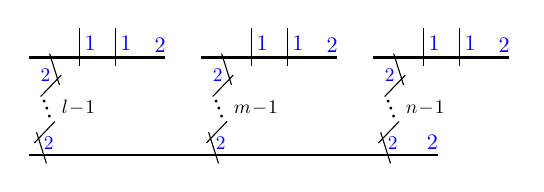
\begin{tikzpicture}[xscale=0.57,yscale=0.62]
\draw[thick,shorten >=2] (-1/3,0)--(89/10,0) node[inner sep=2pt,blue,above left,scale=0.8] {2};
\draw (0,0) 
    ++(0.06,-0.17)--++(-0.22,0.64)++(0.11,-0.24)  
    ++(0,0.02)
      node[blue,scale=0.7,inner sep=1,anchor=west]{2}
    ++(0,-0.02)
    ++(-0.16,0.02)--++(0.46,0.44)++(-0.12,0.08)  
    node{$\cdot$} ++(-0.06,0.16) node{$\cdot$}
    ++(-0.06,0.16) node{$\cdot$}++(0.17,-0.12)    node[auto,inner sep=5,scale=0.7,anchor=west]{$l\!-\!1$}
    ++(-0.25,0.23)--++(0.46,0.44)++(-0.19,0.04)   
    ++(0,-0.05)
      node[blue,scale=0.7,inner sep=1,anchor=east]{2}
    ++(0,0.05)
    ++(0.19,-0.04)++(-0.04,-0.2)--++(-0.22,0.64);
\draw[thick,shorten >=2] (-1/3,2)--(17/6,2) node[inner sep=2pt,blue,above left,scale=0.8] {2};
\draw[shorten <=-3pt] (4/5,2)--node[inner sep=2pt,scale=0.8,blue,right] {1} (4/5,13/5);
\draw[shorten <=-3pt] (8/5,2)--node[inner sep=2pt,scale=0.8,blue,right] {1} (8/5,13/5);
\draw (23/6,0) 
    ++(0.06,-0.17)--++(-0.22,0.64)++(0.11,-0.24)  
    ++(0,0.02)
      node[blue,scale=0.7,inner sep=1,anchor=west]{2}
    ++(0,-0.02)
    ++(-0.16,0.02)--++(0.46,0.44)++(-0.12,0.08)  
    node{$\cdot$} ++(-0.06,0.16) node{$\cdot$}
    ++(-0.06,0.16) node{$\cdot$}++(0.17,-0.12)    node[auto,inner sep=5,scale=0.7,anchor=west]{$m\!-\!1$}
    ++(-0.25,0.23)--++(0.46,0.44)++(-0.19,0.04)   
    ++(0,-0.05)
      node[blue,scale=0.7,inner sep=1,anchor=east]{2}
    ++(0,0.05)
    ++(0.19,-0.04)++(-0.04,-0.2)--++(-0.22,0.64);
\draw[thick,shorten >=2] (7/2,2)--(20/3,2) node[inner sep=2pt,blue,above left,scale=0.8] {2};
\draw[shorten <=-3pt] (139/30,2)--node[inner sep=2pt,scale=0.8,blue,right] {1} (139/30,13/5);
\draw[shorten <=-3pt] (163/30,2)--node[inner sep=2pt,scale=0.8,blue,right] {1} (163/30,13/5);
\draw (23/3,0) 
    ++(0.06,-0.17)--++(-0.22,0.64)++(0.11,-0.24)  
    ++(0,0.02)
      node[blue,scale=0.7,inner sep=1,anchor=west]{2}
    ++(0,-0.02)
    ++(-0.16,0.02)--++(0.46,0.44)++(-0.12,0.08)  
    node{$\cdot$} ++(-0.06,0.16) node{$\cdot$}
    ++(-0.06,0.16) node{$\cdot$}++(0.17,-0.12)    node[auto,inner sep=5,scale=0.7,anchor=west]{$n\!-\!1$}
    ++(-0.25,0.23)--++(0.46,0.44)++(-0.19,0.04)   
    ++(0,-0.05)
      node[blue,scale=0.7,inner sep=1,anchor=east]{2}
    ++(0,0.05)
    ++(0.19,-0.04)++(-0.04,-0.2)--++(-0.22,0.64);
\draw[thick,shorten >=2] (22/3,2)--(21/2,2) node[inner sep=2pt,blue,above left,scale=0.8] {2};
\draw[shorten <=-3pt] (127/15,2)--node[inner sep=2pt,scale=0.8,blue,right] {1} (127/15,13/5);
\draw[shorten <=-3pt] (139/15,2)--node[inner sep=2pt,scale=0.8,blue,right] {1} (139/15,13/5);
\end{tikzpicture}
\end{document}
